\documentclass[%
%%% PARA ESCOLHER O ESTILO TIRE O SIMBOLO %(COMENTÁRIO)
%SemVinculoColorido,
%SemFormatacaoCapitulo,
%SemFolhaAprovacao,
%SemImagens,
%CitacaoNumerica, %% o padrão é citação tipo autor-data
%PublicacaoDissOuTese, %% (é também o "default") com ficha catal. e folha de aprovação em branco. Caso tenha lista de símbolos e lista de siglas e abreviaturas retirar os comentários dos arquivos siglas.tex e abreviaturasesiglas.tex. Retirar também os comentários indicados nesse arquivo, nos includes
PublicacaoArtigoOuRelatorio, %% texto sequencial, sem quebra de páginas nem folhas em branco
%PublicacaoProposta, %% igual tese/dissertação, mas sem ficha catal. e fol. de aprov.
%PublicacaoLivro, %% com capítulos
%PublicacaoLivro,SemFormatacaoCapitulo, %% sem capítulos
english,portuguese %% para os documentos em Português com abstract.tex em Inglês
%portuguese,english %% para os documentos em Inglês com abstract.tex em Português
,LogoINPE% comentar essa linha para fazer aparecer o logo do Governo
%,CCBYNC	% as opções de licença são: CCBY, CCBYSA, CCBYND, CCBYNC, CCBYNCSA, CCBYNCND, GPLv3 e INPECopyright
]{tdiinpe}
%]{../../../../../iconet.com.br/banon/2008/03.25.01.19/doc/tdiinpe}

% PARA EXIBIR EM ARIAL TIRAR O COMENTÁRIO DAS DUAS LINHAS SEGUINTES
%\renewcommand{\rmdefault}{phv} % Arial
%\renewcommand{\sfdefault}{phv} % Arial

% PARA PUBLICAÇÕES EM INGLÊS:
% renomear o arquivo: abnt-alf.bst para abnt-alfportuguese.bst
% renomear o arquivo: abnt-alfenglish.bst para abnt-alf.bst


%%%%%%%%%%%%%%%%%%%%%%%%%%%%%%%%%%%%%%%%%%%%%
%%% Pacotes já previamente carregados:      %
%%%%%%%%%%%%%%%%%%%%%%%%%%%%%%%%%%%%%%%%%%%%%%%%%%%%%%%%%%%%%%%%%%%%%%%%
%%% ifthen,calc,graphicx,color,inputenc,babel,hyphenat,array,setspace, %
%%% bigdelim,multirow,supertabular,tabularx,longtable,lastpage,lscape, %
%%% rotate,caption2,amsmath,amssymb,amsthm,subfigure,tocloft,makeidx,  %
%%% eso-pic,calligra,hyperref,ae,fontenc                               %
%%%%%%%%%%%%%%%%%%%%%%%%%%%%%%%%%%%%%%%%%%%%%%%%%%%%%%%%%%%%%%%%%%%%%%%%
%%% insira neste campo, comandos de LaTeX %%%
%%% \usepackage{_exemplo_}
% etc.
\usepackage{xcolor}
\usepackage{rotating}
\usepackage{dsfont}
\usepackage{listings}
\usepackage{booktabs}

\lstset{language=c} 
\lstset{language=C, literate={-}{-}1}

\definecolor{codegreen}{rgb}{0,0.6,0}
\definecolor{codegray}{rgb}{0.3,0.3,0.3}
\definecolor{codepurple}{rgb}{0.58,0,0.82}
\definecolor{backcolour}{rgb}{0.95,0.95,0.92}

\lstdefinestyle{mystyle}{
    backgroundcolor=\color{backcolour},   
    commentstyle=\color{codegreen},
    keywordstyle=\color{magenta},
    numberstyle=\tiny\color{codegray},
    stringstyle=\color{codepurple},
    basicstyle=\ttfamily\footnotesize,
    breakatwhitespace=false,         
    breaklines=true,                 
    captionpos=b,                    
    keepspaces=true,                 
    numbers=left,                    
    numbersep=5pt,                  
    showspaces=false,                
    showstringspaces=false,
    showtabs=false,                  
    tabsize=2
}

\lstdefinestyle{mystyle2}{
    backgroundcolor=\color{backcolour},   
    commentstyle=\color{codegreen},
    keywordstyle=\color{magenta},
    stringstyle=\color{codepurple},
    basicstyle=\ttfamily\footnotesize,
    breakatwhitespace=false,         
    breaklines=true,                 
    captionpos=b,                    
    keepspaces=true,                                             
    showspaces=false,                
    showstringspaces=false,
    showtabs=false,                  
    tabsize=2
}
%%%%%%%%%%%%%%%%%%%%%%%%%%%%%%%%%%%%%%%%%%%%%

%\watermark{Revisão No. ##} %% use o comando \watermark para identificar a versão de seu documento
%% comente este comando quando for gerar a versão final

%%%%%%%%%%%%%%%%%%%CAPA%%%%%%%%%%%%%%%%%%%%%%%%%%%%%%%%
%\serieinpe{INPE-NNNNN-TDI/NNNN} %% não mais usado

\titulo{Projeto Fourier}
\title{Projeto Fourier} %% 
\author{Leonardo Sattler Cassará} %% coloque o nome do(s) autor(es)
\descriccao{Relatório apresentado à Prof.\textsuperscript{a} Margarete O. Domingues como atividade do curso Análise Wavelet I.}
\repositorio{} %% repositório onde está depositado este documento - na omissão, será preenchido pelo SID
\tipoDaPublicacao{}	%% tipo da publicação (NTC, RPQ, PRP, MAN, PUD, TDI, TAE e PRE) na ausência do número de série INPE, caso contrário deixar vazio
\IBI{} %% IBI (exemplo: J8LNKAN8PW/36CT2G2) quando existir, caso contrário o nome do repositório onde está depositado o documento

\date{25 de setembro de 2020}%ano da publicação

%%%%%%%%%%%%%%%%%%%%%%%%%%VERSO DA CAPA%%%%%%%%%%%%%%%%%%%%%%%%%%%%%%%%%%%%%%%%%%%%%%%
\tituloverso{}
\descriccaoverso{}

\descriccaoversoA{}

%%%%%%%%%%%%%%%%%%%FOLHA DE ROSTO

%%%%%%%%%%%%%%%FICHA CATALOGRÁFICA
%% NÃO PREENCHER - SERÁ PREENCHIDO PELO SID

\cutterFICHAC{Cutter}
\autorUltimoNomeFICHAC{Sobrenome, Nomes} %% exemplo: Fuckner, Marcus André
\autorFICHAC {Nome Completo do Autor1; Nome Completo do Autor2} %% Campo opcional (se não usado prevalece \author)
\tituloFICHAC{Titulo da publicação}
\instituicaosigla{INPE}
\instituicaocidade{São José dos Campos}
\paginasFICHAC{\pageref{numeroDePáginasDoPretexto} + \pageref{LastPage}} %% número total de páginas
%\serieinpe{INPE-00000-TDI/0000} %% não mais usado
\palavraschaveFICHAC{1.~Palavra chave. 2.~Palavra chave 3.~Palavra chave. 4.~Palavra chave. 5.~Palavra chave  I.~\mbox{Título}.} %% recomenda-se pelo menos 5 palavras-chaves - \mbox{} é para evitar hifenização 
\numeroCDUFICHAC{000.000} %% número do CDU 

% Nota da ficha (para TD)
\tipoTD{Dissertação ou Tese} % Dissertação ou Tese
\cursoFA{Mestrado ou Doutorado em Nome do Curso}
\instituicaoDefesa{Instituto Nacional de Pesquisas Espaciais}
\anoDefesa{AAAA} % ano de defesa 
\nomeAtributoOrientadorFICHAC{Orientador}	% pode ser: Orientador, Orientadora ou Orientadores
\valorAtributoOrientadorFICHAC{José da Silva} % nome(s) completo(s)

%%%%%%%%%%%%%%%FOLHA DE APROVAÇAO PELA BANCA EXAMINADORA
\tituloFA{\textbf{ATENÇÃO! A FOLHA DE APROVAÇÃO SERÁ INCLUIDA POSTERIORMENTE.}}
%\cursoFA{\textbf{}}
\candidatoOUcandidataFA{}
\dataAprovacaoFA{}
\membroA{}{}{}
\membroB{}{}{}
\membroC{}{}{}
\membroD{}{}{}
\membroE{}{}{}
\membroF{}{}{}
\membroG{}{}{}
\ifpdf

%%%%%%%%%%%%%%NÍVEL DE COMPRESSÃO {0 -- 9}
\pdfcompresslevel 9
\fi
%%% define em 80% a largura das figuras %%%
\newlength{\mylenfig} 
\setlength{\mylenfig}{0.8\textwidth}
%%%%%%%%%%%%%%%%%%%%%%%%%%%%%%%%%%%%%%%%%%%

%%%%%%%%%%%%%%COMANDOS PESSOAIS
\newcommand{\vetor}[1]{\mathit{\mathbf{#1}}} %% faça as modificações pertinentes no arquivo configuracao.tex

\makeindex  %% não alterar, gera INDEX, caso haja algum termo indexado no texto

\begin{document} %% início do documento %% não mexer

%\marcaRegistrada{}	% comando opcional usado para informar abaixo da ficha catalográfica sobre marca registrada
%\marcaRegistrada{Informar aqui sobre marca registrada (a modificação desta linha deve ser feita no arquivo publicacao.tex).}

\maketitle  %% não alterar, gera páginas obrigatórias (folha de rosto, ficha catalográfica e folha de aprovação), automaticamente

%%% Comente as linhas opcionais abaixo caso não as deseje
%\include{./docs/epigrafe} %% Opcional
%\include{./docs/dedicatoria} %% Opcional
%\include{./docs/agradecimentos} %% Opcional
%%%%%%%%%%%%%%%%%%%%%%%%%%%%%%%%%%%%%%%%%%%%%%%%%%%%%%%%%%%%%%%%%%%%%%%%%%%%%%%%
% RESUMO %% obrigatório

\begin{resumo}

%% neste arquivo resumo.tex
%% o texto do resumo e as palavras-chave têm que ser em Português para os documentos escritos em Português
%% o texto do resumo e as palavras-chave têm que ser em Inglês para os documentos escritos em Inglês
%% os nomes dos comandos \begin{resumo}, \end{resumo}, \palavraschave e \palavrachave não devem ser alterados

\hypertarget{estilo:resumo}{} %% uso para este Guia

Neste trabalho, dados do fluxo solar na faixa de 10.7 cm foram analisados no contexto da Análise de Fourier. Três conjuntos de dados, médias diárias, médias de 27 dias e médias anuais foram explorados através da biblioteca \texttt{numpy} (da linguagem \texttt{Python}) com a rotina \texttt{numpy.fft}. O espectro de potência dos sinais foi extraído e seu resultado discutido à luz do conhecido ciclo de atividade solar, cujo período é de onze anos. O objetivo deste projeto é a familiarização de técnicas para análise de séries temporais através do formalismo de Fourier, contribuindo para a assimilação de conceitos relevantes à disciplina Análise Wavelet I.

\palavraschave{%
	\palavrachave{Fluxo solar}%
	\palavrachave{Transformada de Fourier}%
	\palavrachave{Espectro de potência}%
	\palavrachave{Análise de sinal}%
	\palavrachave{Séries temporais}%
}
 
\end{resumo} %% obrigatório
%\include{./docs/abstract} %% obrigatório

\includeListaFiguras %% obrigatório caso haja mais de 3 figuras, gerado automaticamente
%\includeListaTabelas %% obrigatório caso haja mais de 3 tabelas, gerado automaticamente

%\include{./docs/abreviaturasesiglas} %% opcional %% altere o arquivo siglaseabreviaturas.tex

%\include{./docs/simbolos} %% opcional %% altere o arquivo simbolos.tex

\includeSumario  %% obrigatório, gerado automaticamente

\newpage
\inicioIntroducao %% não altere este comando

%%%%%%%%%%%%%%%%%%%%%%%%%%%%%%%%%%%%%%%%%%%%%%%%%%%%%%%%%%%%%%%%%%%%%%%%%%%%%%%

\chapter{INTRODUÇÃO}

O fluxo solar na faixa de 10.7 cm (doravante chamado F10.7) é uma medida da intensidade da emissão do sol na faixa do rádio, mais precisamente em 10.7 cm (ou 2800 MHz). Este índice é um indicador da atividade magnética do Sol, fornecendo informações da atividade solar no ultravioleta e raio-X. Por isso, esse índice é muito relevante em ramos como astrofísica, meteoroglogia e geofísica. Com aplicações em modelagem climática, seu monitoramento é importante para a manutenção dos sistemas de comunicação via satélite \cite{huang2009forecast}. 

Em conjunto com os dados de manchas solares, F10.7 é um dos indicadores mais usados para previsão da atividade solar. Por esse motivo, muitos estudos objetivando predição do clima espacial o utilizam como parâmetro de input. Por exemplo, \citeonline{mordvinov1986prediction} utilizou autorregressão multiplicativa para predição mensal dos valores de F10.7. \citeonline{dmitriev1999solar} aplicaram redes neurais para a predição. Por sua vez, \citeonline{zhong2005application} aplicou análise espectral para prever os valores de F10.7. Já \citeonline{bruevich2014study} aplicou análise Wavelet sobre as médias mensais desse dado para análise da série temporal.

A análise espectral é um método para representar um sinal como a combinação linear de funções periódicas. Ela faz parte de uma família de técnicas chamadas de Análise de Fourier. No presente trabalho, os dados do índice F10.7 são analisados no contexto da Análise de Fourier. Este manuscrito está assim organizado: na Seção 2 os dados e os tratamentos nele realizados são descritos; na Seção 3 é feita uma recapitulação da Análise de Fourier; na Seção 4 os resultados são apresentados com uma breve discussão; na Seção 5 são oferecidas as considerações finais do autor.
 %% 1o capítulo, começo do texto

%%%%%%%%%%%%%%%%%%%%%%%%%%%%%%%%%%%%%%%%%%%%%%%%%%%%%%%%%%%%%%%%%%%%%%%%%%%%%%%

\chapter{OS DADOS}

Como descrito na seção anterior, os dados aqui analisados dizem respeito ao fluxo solar no comprimento de onda de 10.7 cm que, junto com o número de manchas solares, é um dos dados de mais longo registro da atividade solar - o início sistemático de sua observação se deu em 1947 \cite{tapping201310}. Esta quantidade é expressa em unidades de fluxo solar (ou sfu, do inglês \textit{solar flux unit}), onde 1 sfu = 10$^{-22}$Wm$^{-2}$Hz$^{-1}$.

Os dados foram baixados de \url{https://omniweb.gsfc.nasa.gov/form/dx1.html}. Eles dizem respeito à série temporal de 28 de novembro de 1963 a 20 de julho de 2020. Para esta janela temporal, os seguintes dados foram baixados: média dos valores diários (Figura \ref{fig:dailyavg}), média de 27 dias (Figura \ref{fig:27dayavg}) e média anual (Figura \ref{fig:yearluavg}). As Figuras a seguir foram geradas automaticamente pelo portal de acesso aos dados.

%%%%%%%%%%%%%%%%%%%%%%%%%%%%%%%%%%%%%%%%%%%%%%%%%%%%%%%%%%
% DAILY AVERAGES
\begin{figure}[ht!]
	\caption{Médias diárias do índice F10.7.}
	\vspace{0mm}	% acrescentar o espaçamento vertical apropriado entre o título e a borda superior da figura
	\begin{center}
		\resizebox{13cm}{!}{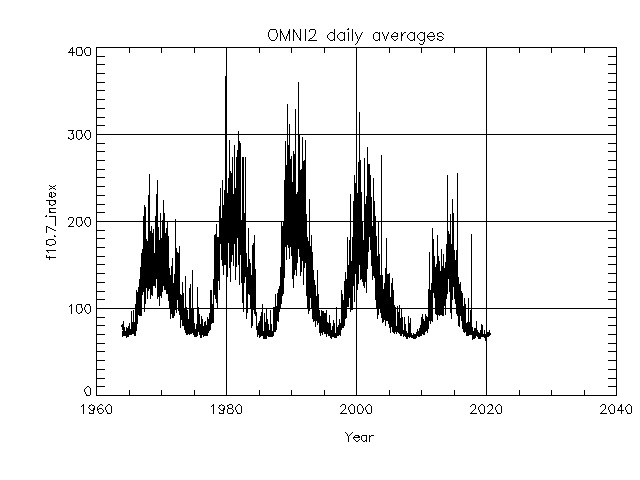
\includegraphics{Figuras/jpg_omni2_daily_wSxReptBqw.jpg}}		
	\end{center}
	\vspace{-2mm}	% acrescentar o espaçamento vertical apropriado entre a borda inferior da figura e a legenda ou a fonte quando não há legenda (o valor pode ser negativo para subir)
	\legenda{Médias das medições diárias do fluxo solar. Visualização fornecida pelo portal utilizado para download. Uma análise direta dos dados indicou presença de saltos com valores 999.9, denotando falhas na aquisição. Variações de grande amplitude ocorrem com maior frequência (diariamente), enquanto uma variação global de amplitude média ocorre na escala de alguns anos. O arquivo possui 20440 registros.}	% legenda - para deixar sem legenda usar comando \legenda{} (nunca deve-se comentar o comando \legenda)
	\label{fig:dailyavg}
	\FONTE{\url{https://omniweb.gsfc.nasa.gov/form/dx1.html}.}	% fonte consultada (elemento obrigatório, mesmo que seja produção do próprio autor)
\end{figure}

%%%%%%%%%%%%%%%%%%%%%%%%%%%%%%%%%%%%%%%%%%%%%%%%%%%%%%%%%%
% 27 DAY AVERAGES
\begin{figure}[ht!]
	\caption{Médias de 27 dias do índice F10.7.}
	\vspace{0mm}	% acrescentar o espaçamento vertical apropriado entre o título e a borda superior da figura
	\begin{center}
		\resizebox{13cm}{!}{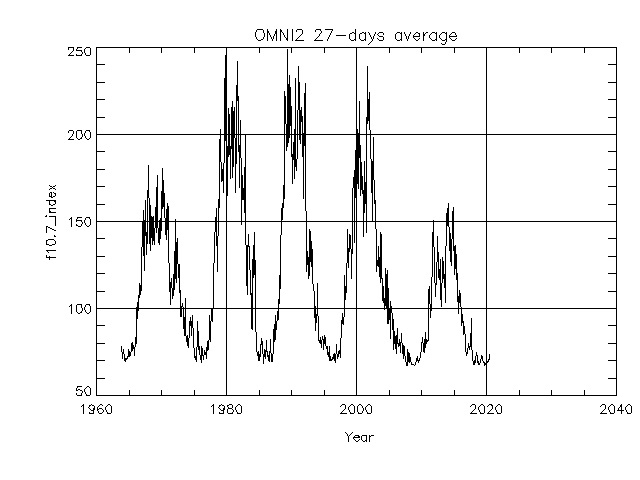
\includegraphics{Figuras/jpg_omni2_27day_bdhxX8pSxb.jpg}}		
	\end{center}
	\vspace{-2mm}	% acrescentar o espaçamento vertical apropriado entre a borda inferior da figura e a legenda ou a fonte quando não há legenda (o valor pode ser negativo para subir)
	\legenda{Médias de 27 dias. As médias tornam o sinal menos oscilatório em pequenas escalas. Ao todo são 672 medições.}	% legenda - para deixar sem legenda usar comando \legenda{} (nunca deve-se comentar o comando \legenda)
	\label{fig:27dayavg}
	\FONTE{\url{https://omniweb.gsfc.nasa.gov/form/dx1.html}.}	% fonte consultada (elemento obrigatório, mesmo que seja produção do próprio autor)
\end{figure}

%%%%%%%%%%%%%%%%%%%%%%%%%%%%%%%%%%%%%%%%%%%%%%%%%%%%%%%%%%
% YEARLY AVERAGES
\begin{figure}[ht!]
	\caption{Médias anuais do índice F10.7.}
	\vspace{0mm}	% acrescentar o espaçamento vertical apropriado entre o título e a borda superior da figura
	\begin{center}
		\resizebox{13cm}{!}{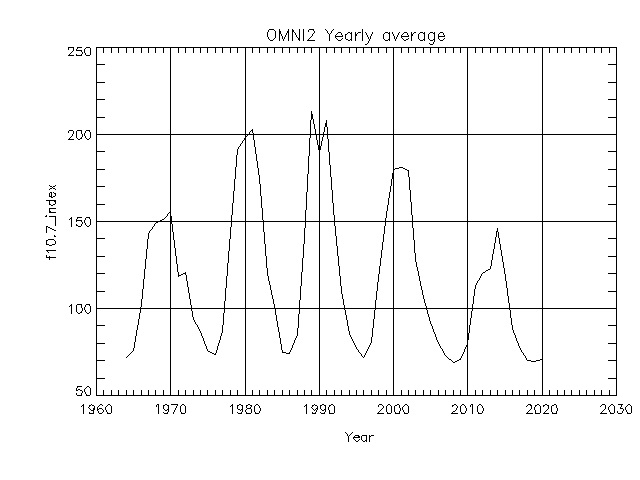
\includegraphics{Figuras/jpg_omni2_yearly_3G19RccK_m.jpg}}		
	\end{center}
	\vspace{-2mm}	% acrescentar o espaçamento vertical apropriado entre a borda inferior da figura e a legenda ou a fonte quando não há legenda (o valor pode ser negativo para subir)
	\legenda{Média anual. Novamente o sinal evidencia sua característica de longo prazo: uma variação sinusoidal com o período de alguns anos. O arquivo possui 56 registros.}	% legenda - para deixar sem legenda usar comando \legenda{} (nunca deve-se comentar o comando \legenda)
	\label{fig:yearluavg}
	\vspace{-3mm}
	\FONTE{\url{https://omniweb.gsfc.nasa.gov/form/dx1.html}.}	% fonte consultada (elemento obrigatório, mesmo que seja produção do próprio autor)
\end{figure}

\begin{figure}[ht!]
	\caption{Tratamento dos dados de média diária.}
	\vspace{0mm}	% acrescentar o espaçamento vertical apropriado entre o título e a borda superior da figura
	\begin{center}
		\resizebox{12cm}{!}{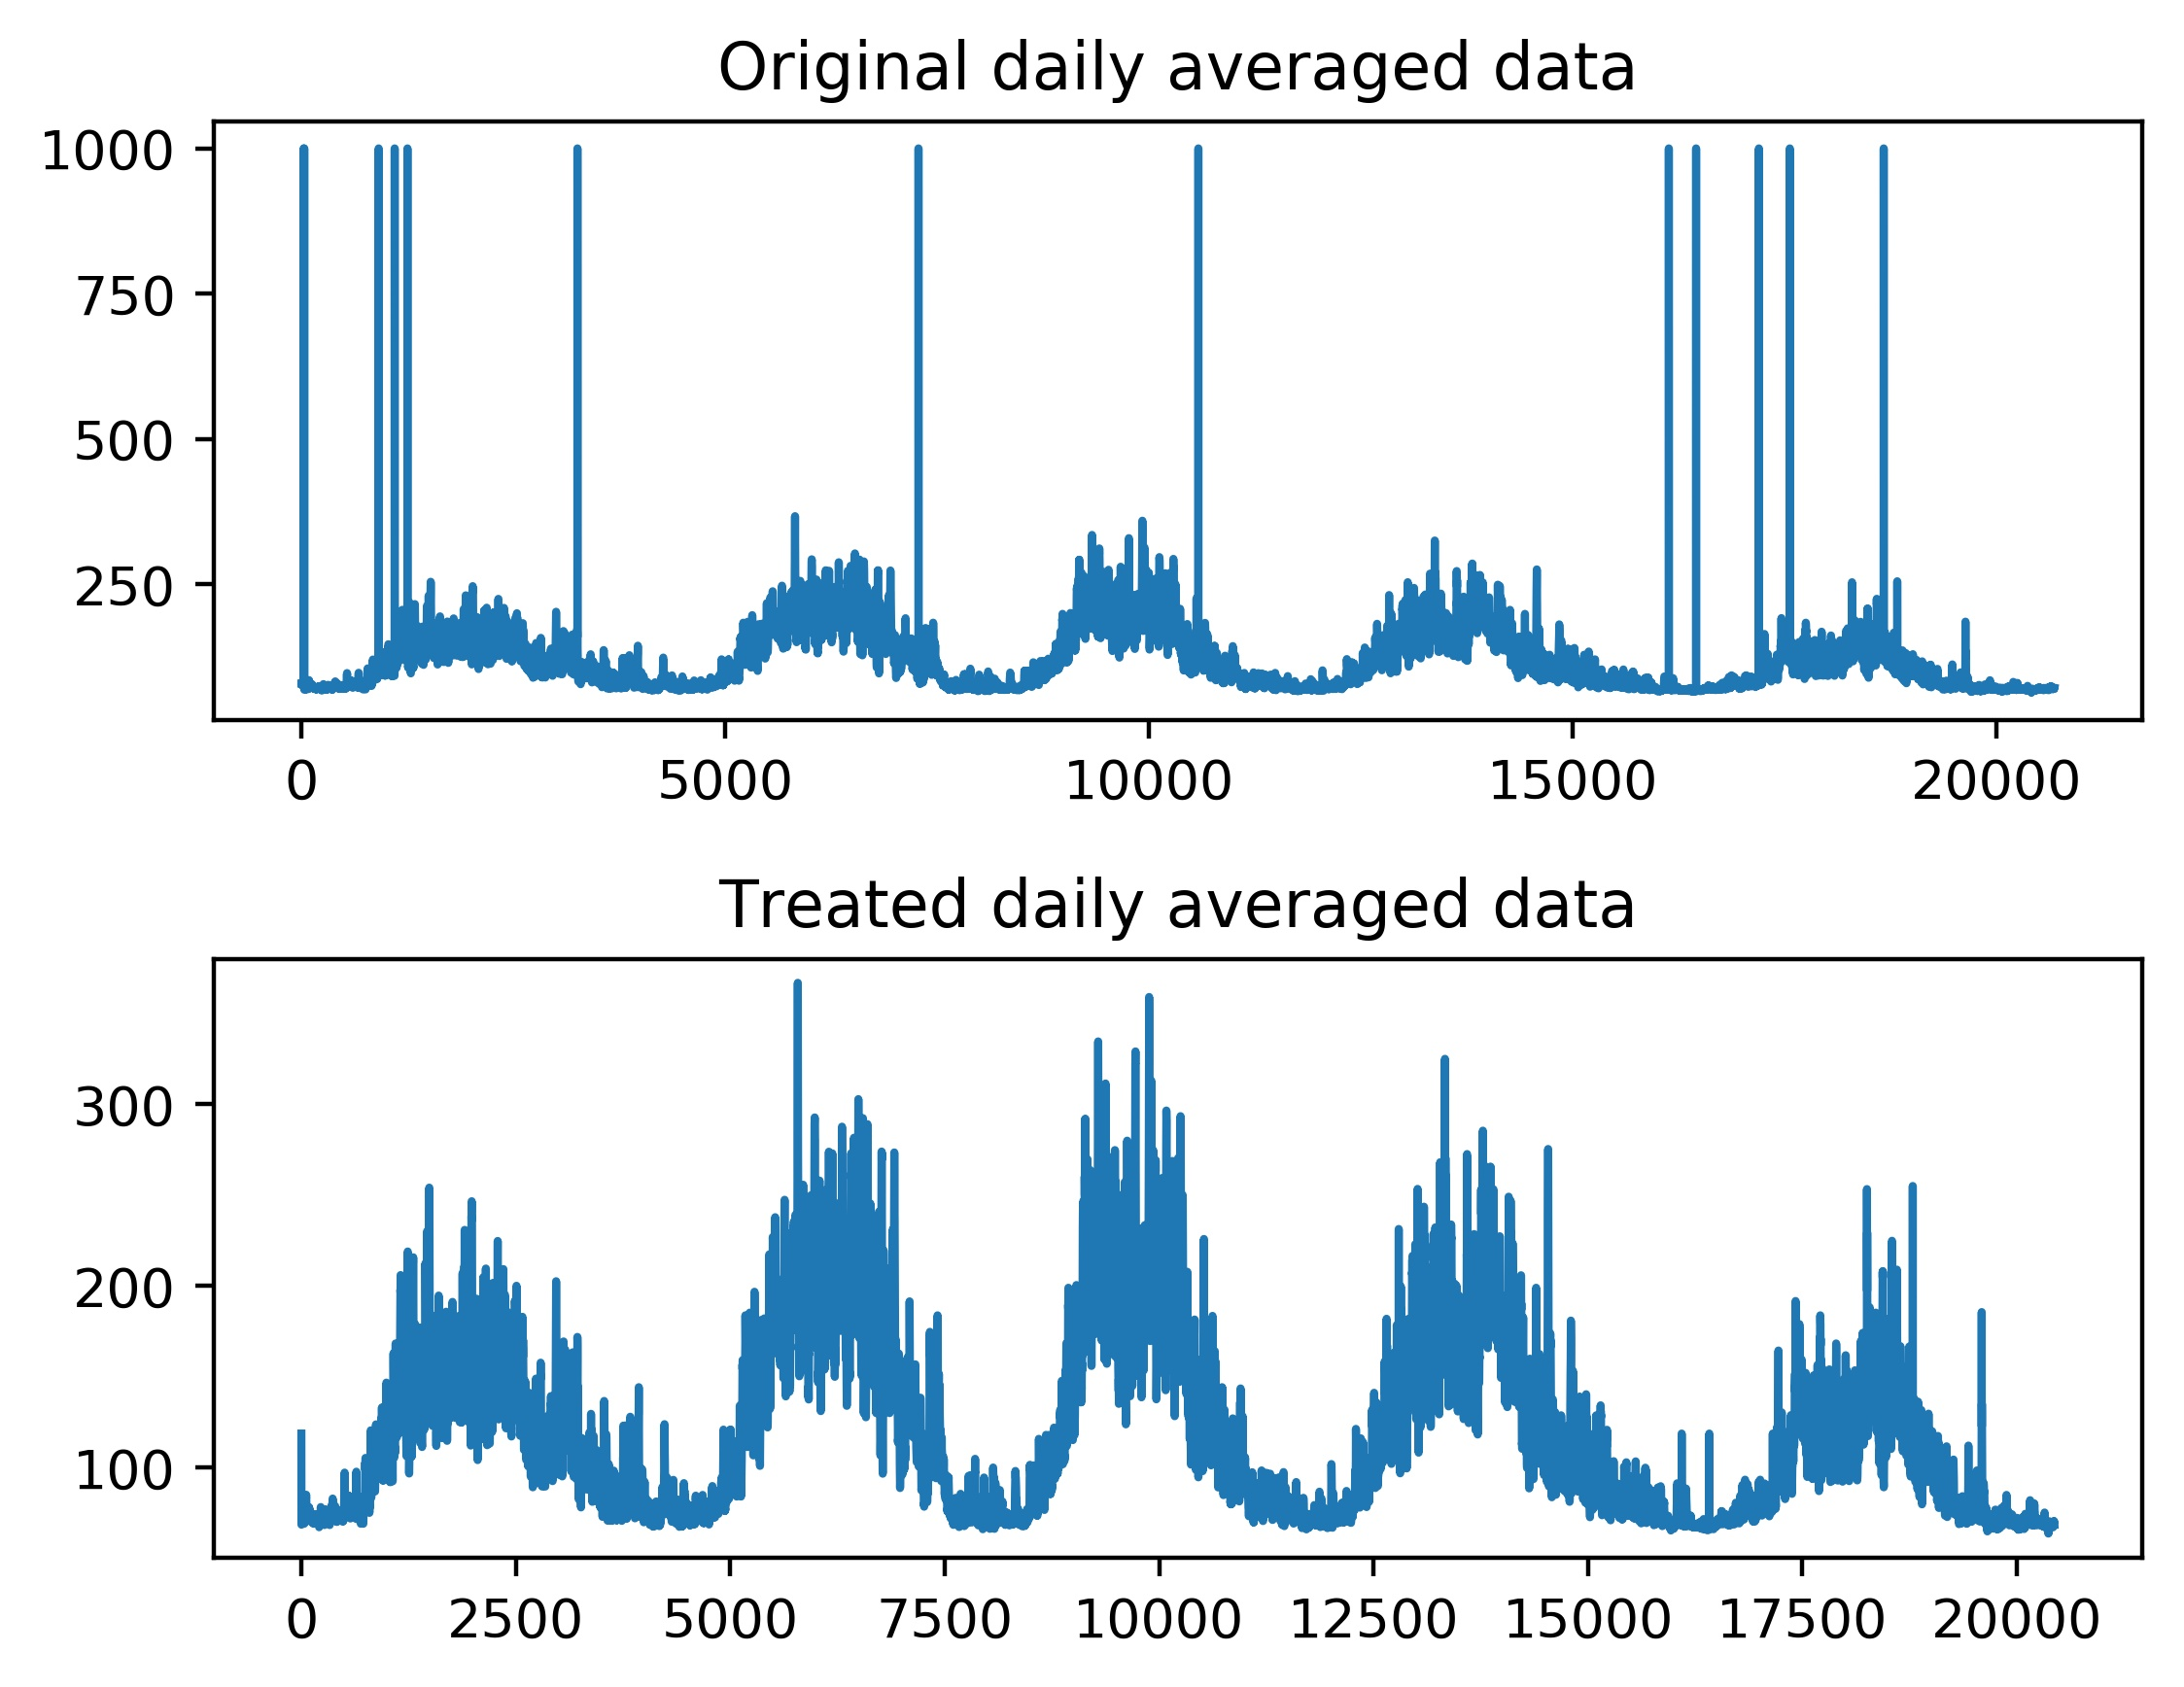
\includegraphics{Figuras/final_2.jpg}}		
	\end{center}
	\vspace{3mm}	% acrescentar o espaçamento vertical apropriado entre a borda inferior da figura e a legenda ou a fonte quando não há legenda (o valor pode ser negativo para subir)
	\legenda{Topo: dados de média diária do fluxo F10.7 conforme baixados, sem nenhum tipo de tratamento; abaixo: mesmos dados após os procedimentos (1), (2) e (3) descritos nesta seção. No plot de baixo, o limite do eixo vertical é reduzido para que um aspecto interessante do sinal possa ser observado: existe uma assimetria na série temporal, que aparenta crescer mais rapidamente e decrescer mais lentamente.}	% legenda - para deixar sem legenda usar comando \legenda{} (nunca deve-se comentar o comando \legenda)
	\label{fig:datavis}
	%\FONTE{\url{https://omniweb.gsfc.nasa.gov/form/dx1.html}.}	% fonte consultada (elemento obrigatório, mesmo que seja produção do próprio autor)
\end{figure}

Os dados diários (Figura \ref{fig:dailyavg}) apresentam valores iguais a 999.9, denotando um valor espúrio a ser lidado antes da análise. Outra característica deste dado é que, para cada ano, existem 365 ou 366 registros, a depender de ser ano bissexto ou não. Para os dados da média de 27 dias (Figura \ref{fig:27dayavg}), existem 13 ou 14 registros, a depender do ano (por motivos intrínsecos ao processo de aquisição dos dados e seus intervalos de medição). Os dados anuais (Figura \ref{fig:yearluavg}) possuem, como esperado, um registro para cada ano. Porém, os anos de 1963 e 2020 de todos os dados dizem respeito a registros incompletos destes anos (apenas de novembro a dezembro de 1963 e de janeiro a julho de 2020). 

Tendo em vista estas características, os dados foram tratados com a seguinte estratégia: (1) a série de 1964 a 2019 foi usada, ignorando-se os valores referentes a 1963 e 2020; (2) os valores 999.9 dos dados de média diária foram substituídos pela média da série; (3) 365 registros de cada ano foram usados nos dados de média diária, ignorando-se o registro extra dos anos bissextos; (4) 12 registros de cada ano foram usados nos dados de média de 27 dias, ignorando-se os demais; (5) o tamanho da série foi reduzida para a maior potência de dois entre zero e o tamanho da série. A Figura \ref{fig:datavis} exibe o dado de média diária antes e depois dos procedimentos (1), (2) e (3) descritos neste parágrafo.  %% 2o capítulo

%%%%%%%%%%%%%%%%%%%%%%%%%%%%%%%%%%%%%%%%%%%%%%%%%%%%%%%%%%%%%%%%%%%%%%%%%%%%%%%

\chapter{METODOLOGIA DE FOURIER}

Análise de Fourier é uma coleção de técnicas para representar funções (ou sinais) gerais como a combinação linear de funções periódicas \cite{li1999fourier}. As ferramentas mais úteis na análise de Fourier são as três transformadas: Séries de Fourier, Transformada Discreta de Fourier (DFT) e Transformada Contínua de Fourier. O processo de calcular as transformadas é chamado de Análise Espectral de Fourier, e esta será a técnica aqui explorada para analisar os dados introduzidos na seção anterior.

Séries de Fourier são úteis para representar funções reais periódicas como uma soma de senos e cossenos com seus respectivos coeficientes (ou pesos). Tais funções sinusoidais formam uma base ortogonal no Espaço de Fourier. As Figuras \ref{fig:FSsqw} e \ref{fig:FSx} ilustram a representação de sinais via Séries de Fourier.

%\vspace{-7mm}
\begin{figure}[ht!]
	\caption{Exemplo Série de Fourier - função periódica.}
	\vspace{1mm}	% acrescentar o espaçamento vertical apropriado entre o título e a borda superior da figura
	\begin{center}
		\resizebox{9cm}{!}{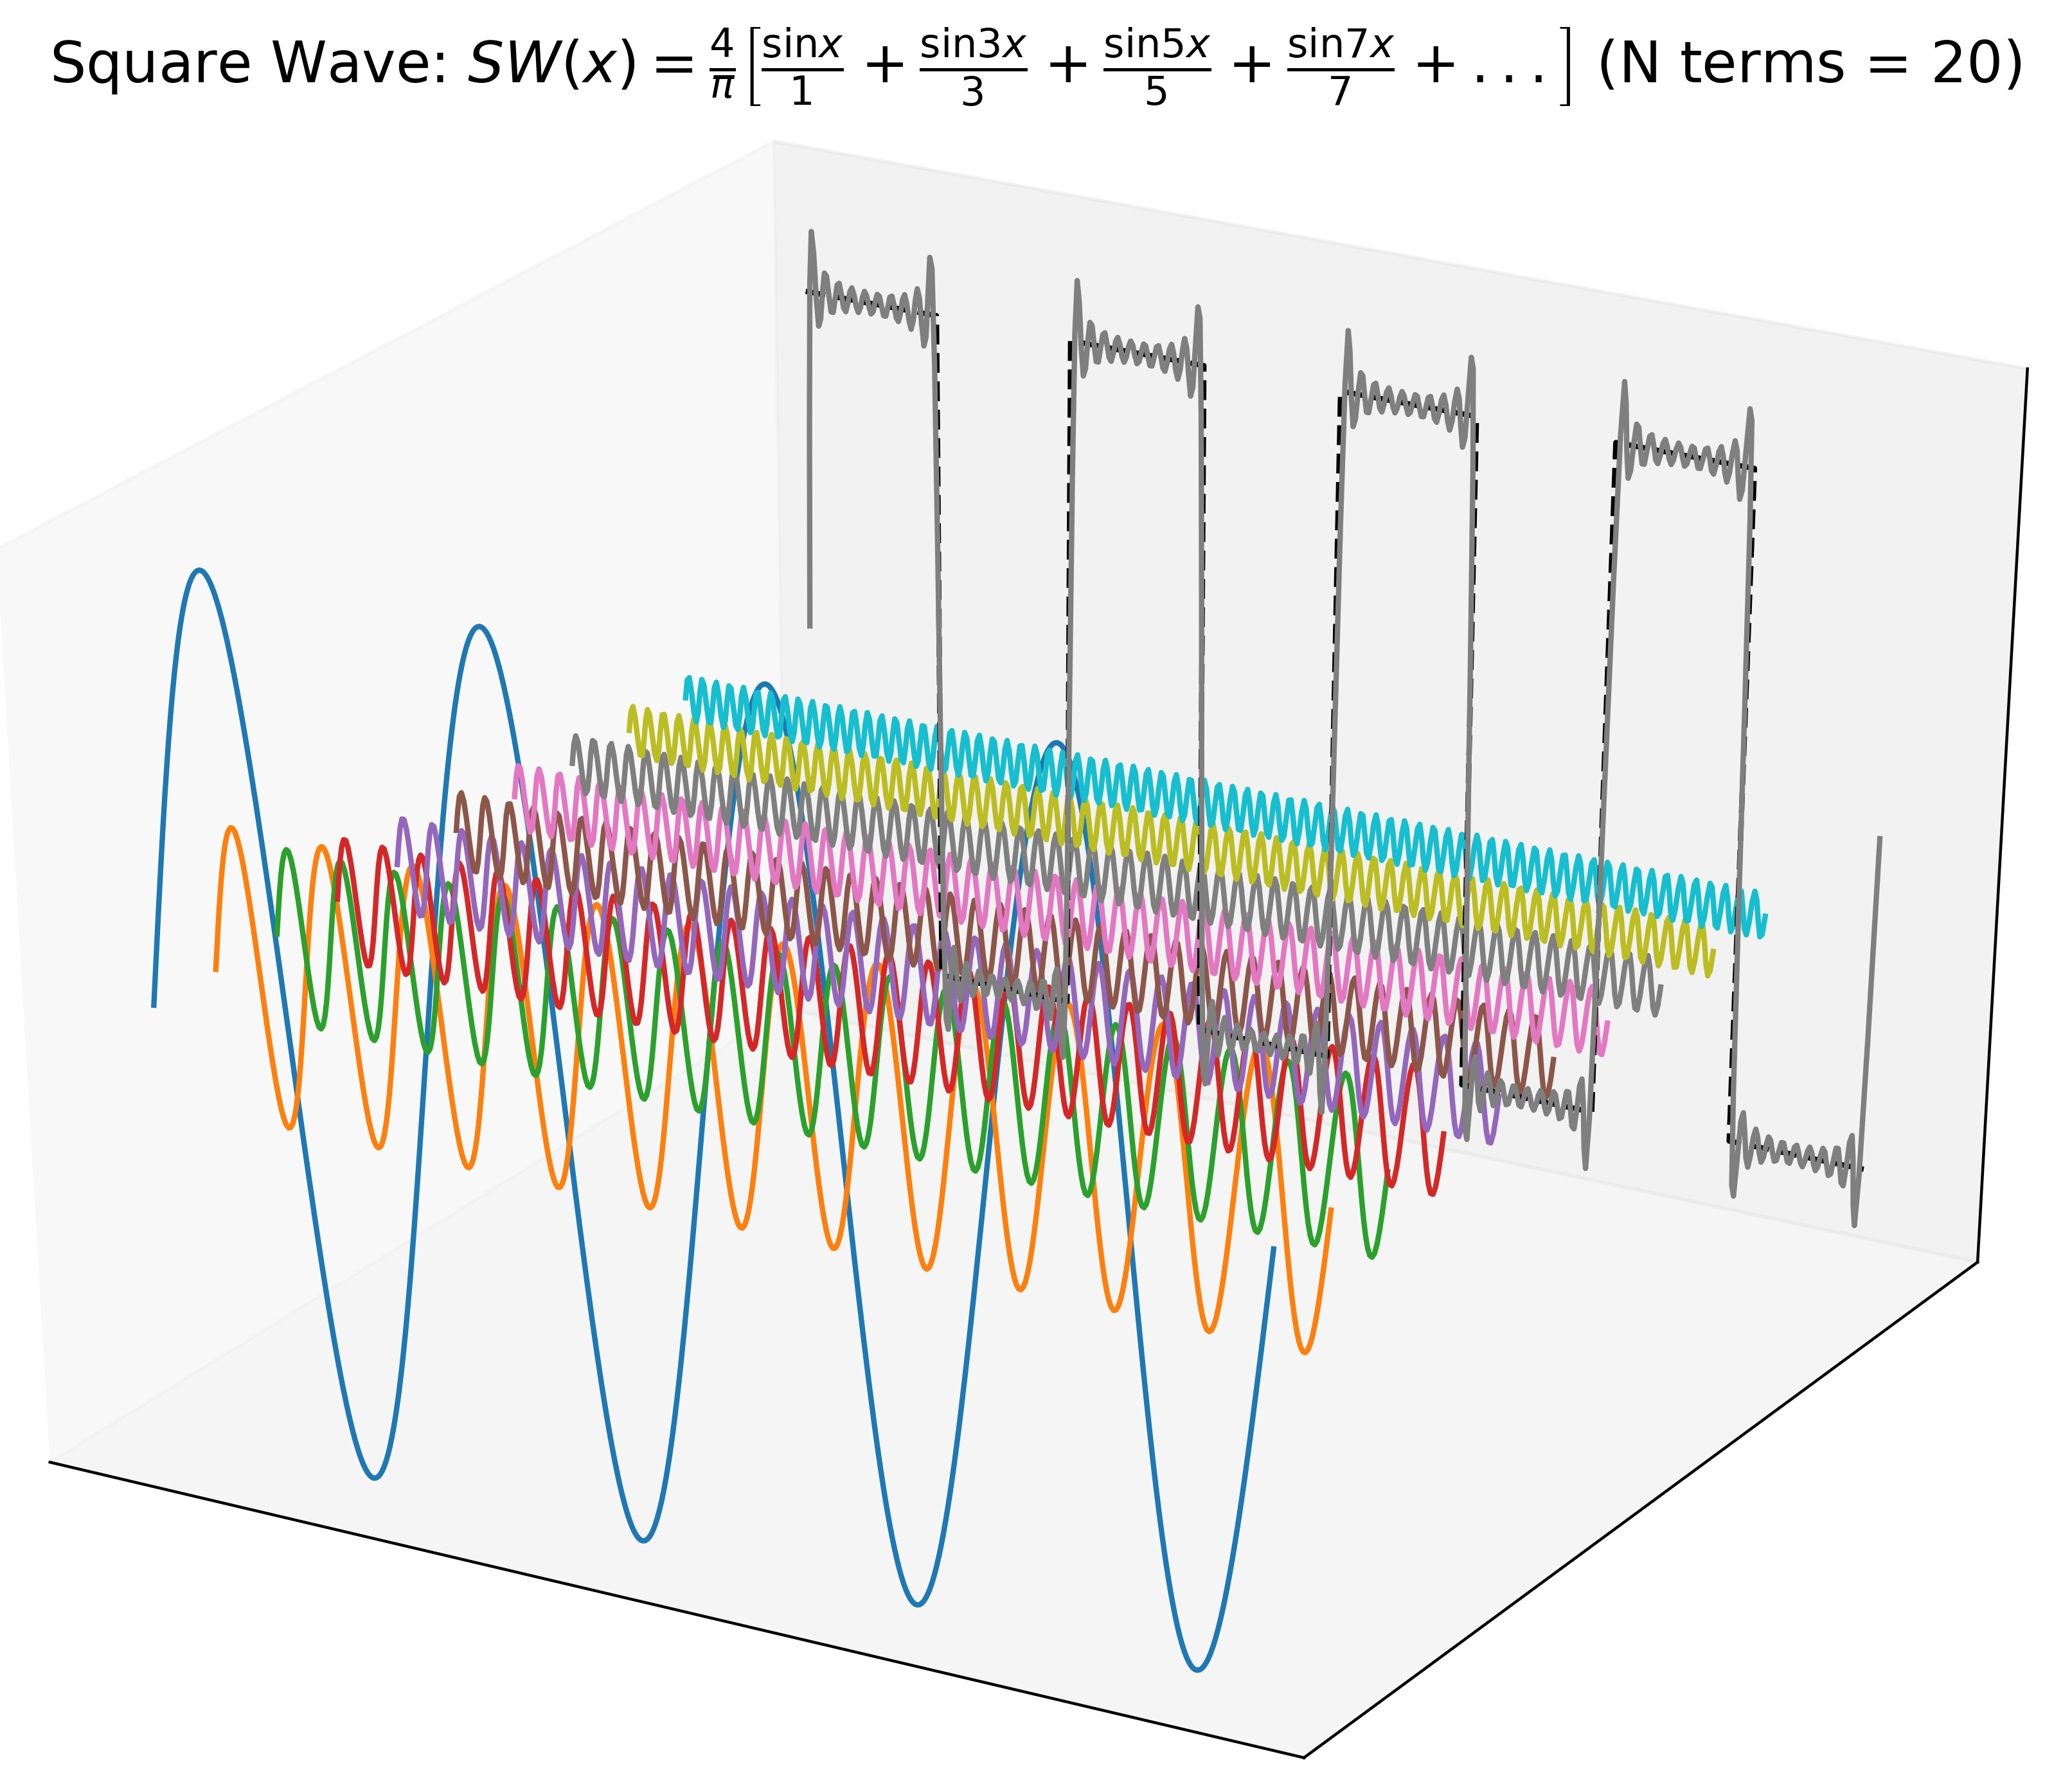
\includegraphics{Figuras/sqw.jpg}}
	\end{center}
	\vspace{0mm}	% acrescentar o espaçamento vertical apropriado entre a borda inferior da figura e a legenda ou a fonte quando não há legenda (o valor pode ser negativo para subir)
	\legenda{Representação de um sinal de perfil quadrado (linha tracejada preta ao fundo) como a soma de senos (linha cinza cheia sobre a linha preta tracejada). No gráfico, os vinte primeiros termos da série são apresentados em sequência.}	% legenda - para deixar sem legenda usar comando \legenda{} (nunca deve-se comentar o comando \legenda)
	\label{fig:FSsqw}
	%\FONTE{\url{https://omniweb.gsfc.nasa.gov/form/dx1.html}.}	% fonte consultada (elemento obrigatório, mesmo que seja produção do próprio autor)
\end{figure}
%\vspace{-12mm}
\begin{figure}[ht!]
	\caption{Exemplo Série de Fourier - função não periódica.}
	\vspace{1mm}	% acrescentar o espaçamento vertical apropriado entre o título e a borda superior da figura
	\begin{center}
		\resizebox{9cm}{!}{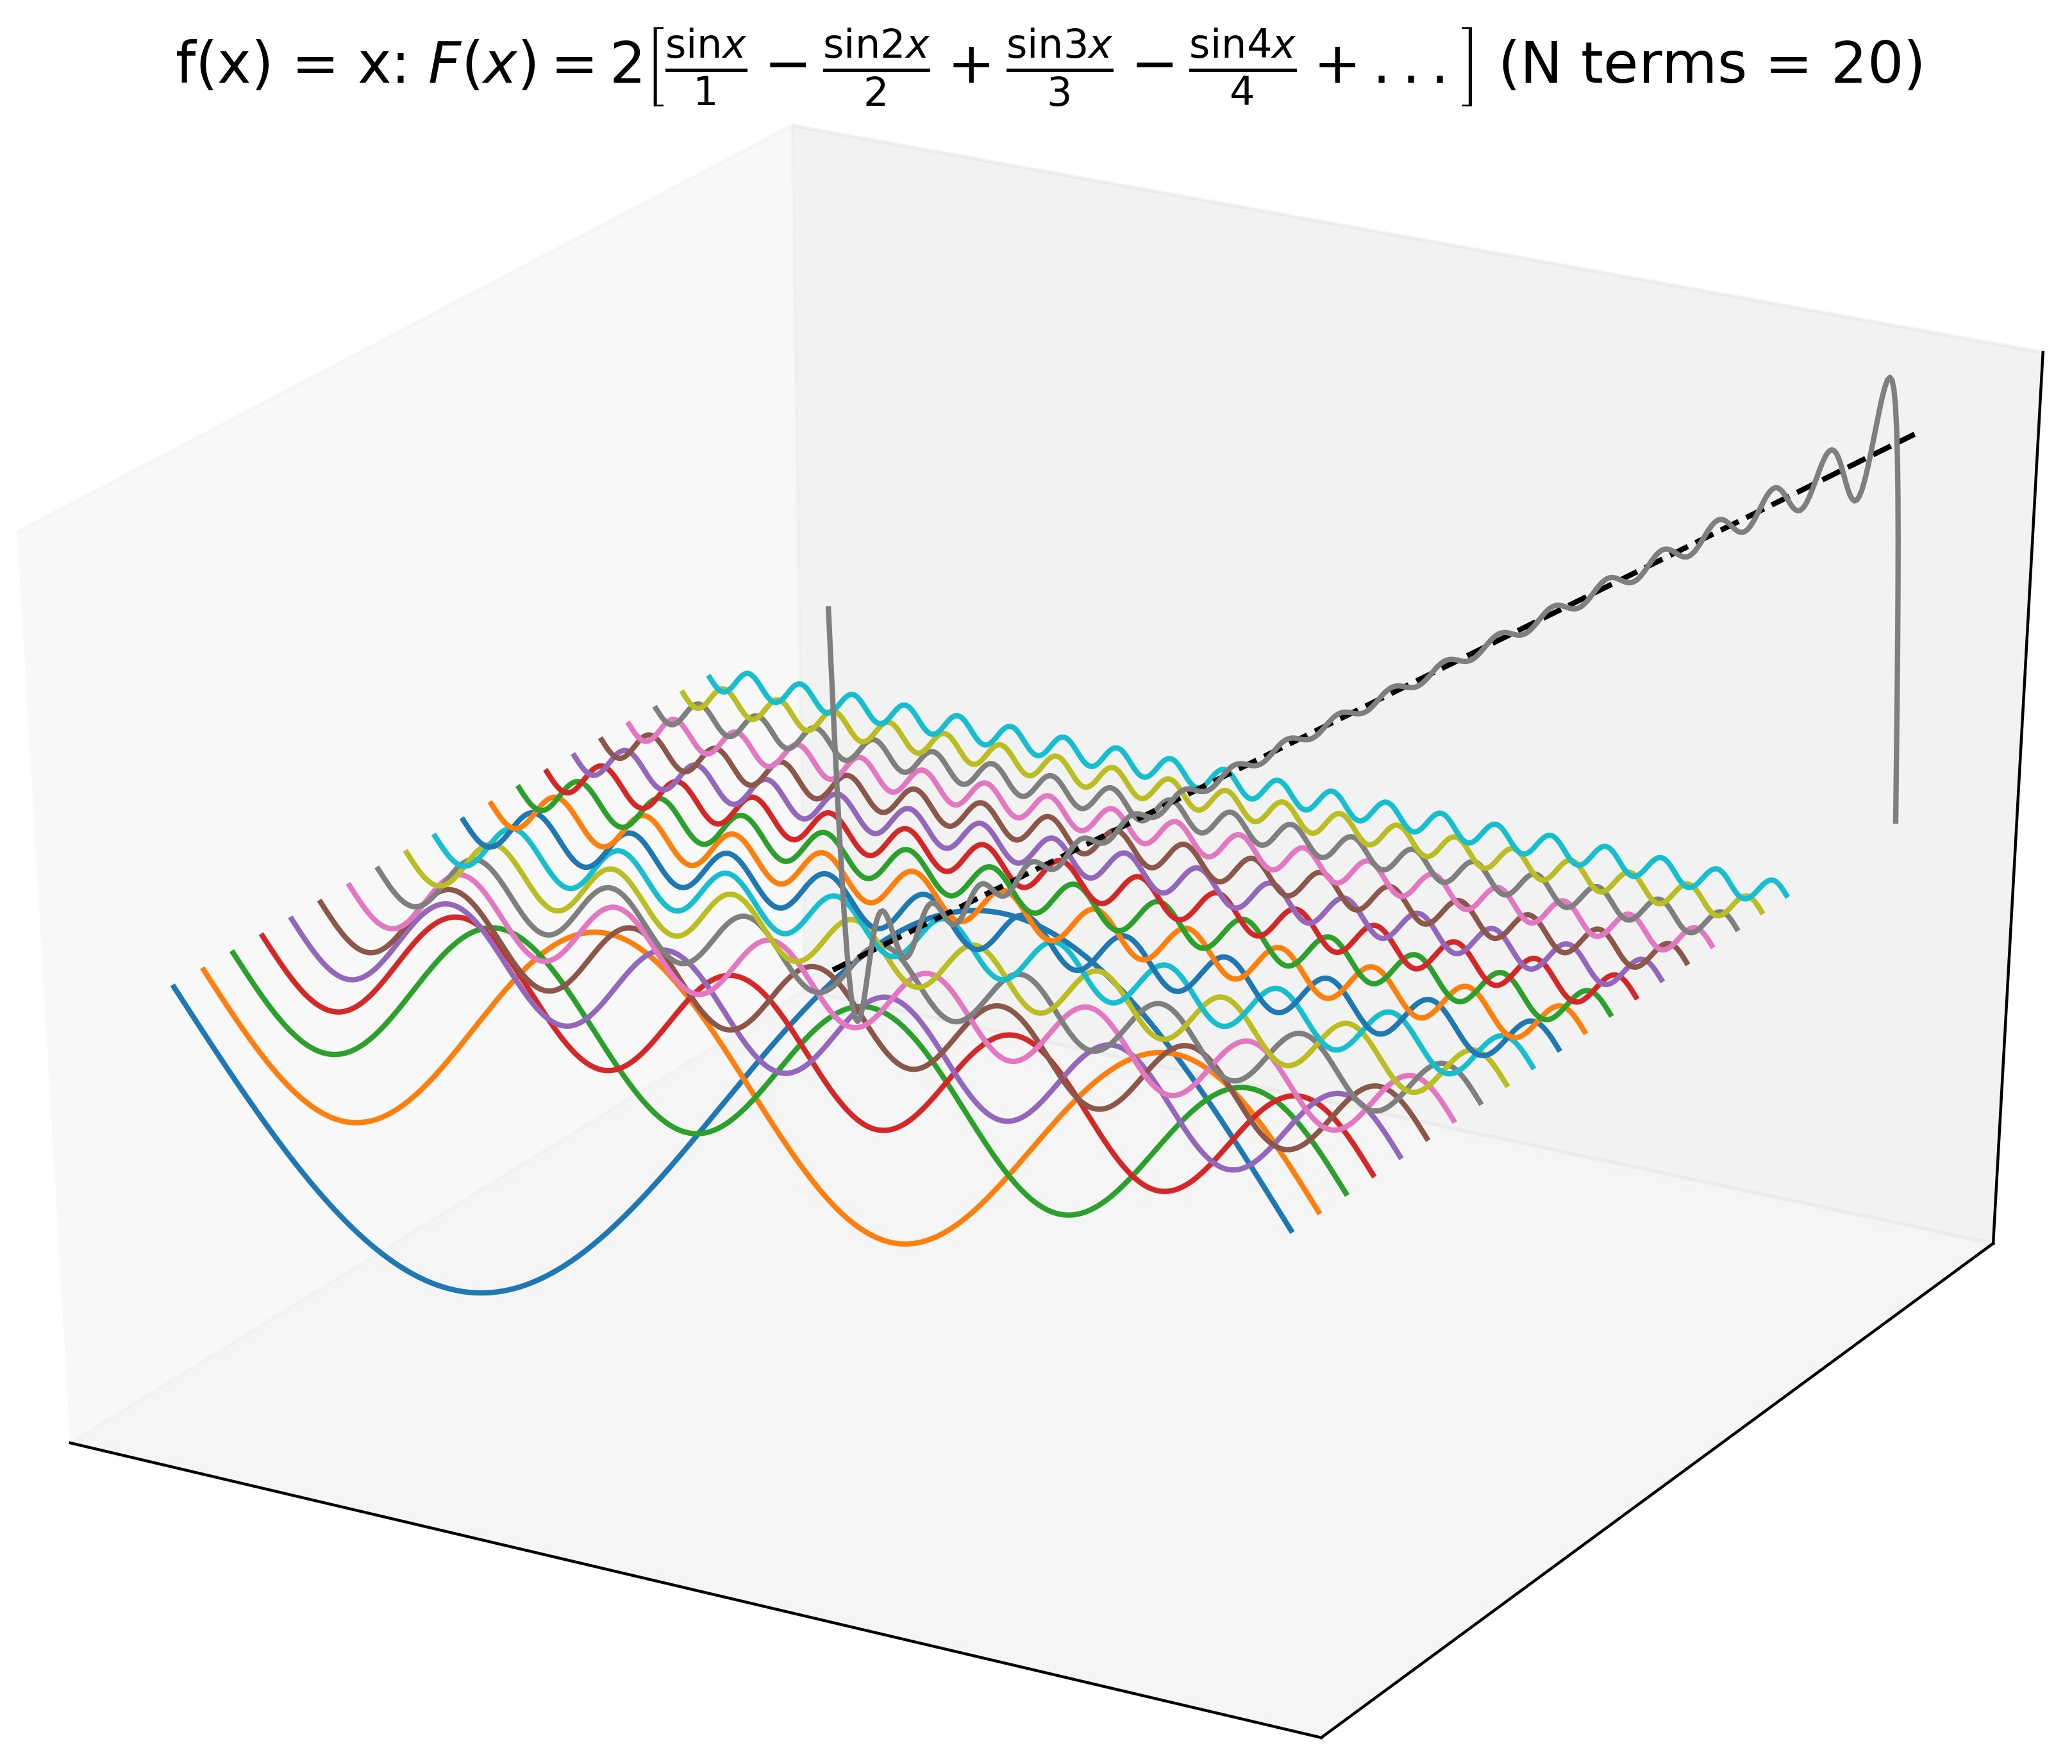
\includegraphics{Figuras/x.jpg}}
	\end{center}
	\vspace{0mm}	% acrescentar o espaçamento vertical apropriado entre a borda inferior da figura e a legenda ou a fonte quando não há legenda (o valor pode ser negativo para subir)
	\legenda{Aplicação das Séries de Fourier, desta vez sobre a função $f(x)= x $. Pode-se observar que mesmo para uma função não necessariamente periódica, é possível a representação em termos de funções sinusoidais. Os vinte primeiros termos foram usados para representar a função.}	% legenda - para deixar sem legenda usar comando \legenda{} (nunca deve-se comentar o comando \legenda)
	\label{fig:FSx}
	%\FONTE{\url{https://omniweb.gsfc.nasa.gov/form/dx1.html}.}	% fonte consultada (elemento obrigatório, mesmo que seja produção do próprio autor)
\end{figure}

A Transformada de Fourier (ou FT, uma abreviação do inglês \textit{Fourier Transform}) não requer que um sinal seja periódico para ser utilizada. Entretanto, ela intrinsecamente considera que o sinal é uma composição de ondas senoidais (bem localizadas na frequência e mal localizadas no tempo). A FT pode ser usada para analisar os conteúdos frequenciais de um sinal, e assim investigar persistências da série. 

Uma aplicação da FT é o chamado espectro de potência. Ele é definido como o módulo quadrado da FT. Ele representa a energia associada a cada conteúdo frequencial. Em outras palavras, a contribuição de cada frequência para a energia total do sinal. A Figura \ref{fig:FT_exemplo} é um exemplo do espectro de potência calculado para os sinais $f_{1}$, $f_{2}$ e uma combinação destes, evidenciando o significado do seu resultado, bem como a característica linear da FT.

\begin{figure}[ht!]
	\caption{Exemplo Transformada de Fourier.}
	\vspace{1mm}	% acrescentar o espaçamento vertical apropriado entre o título e a borda superior da figura
	\begin{center}
		\resizebox{15cm}{!}{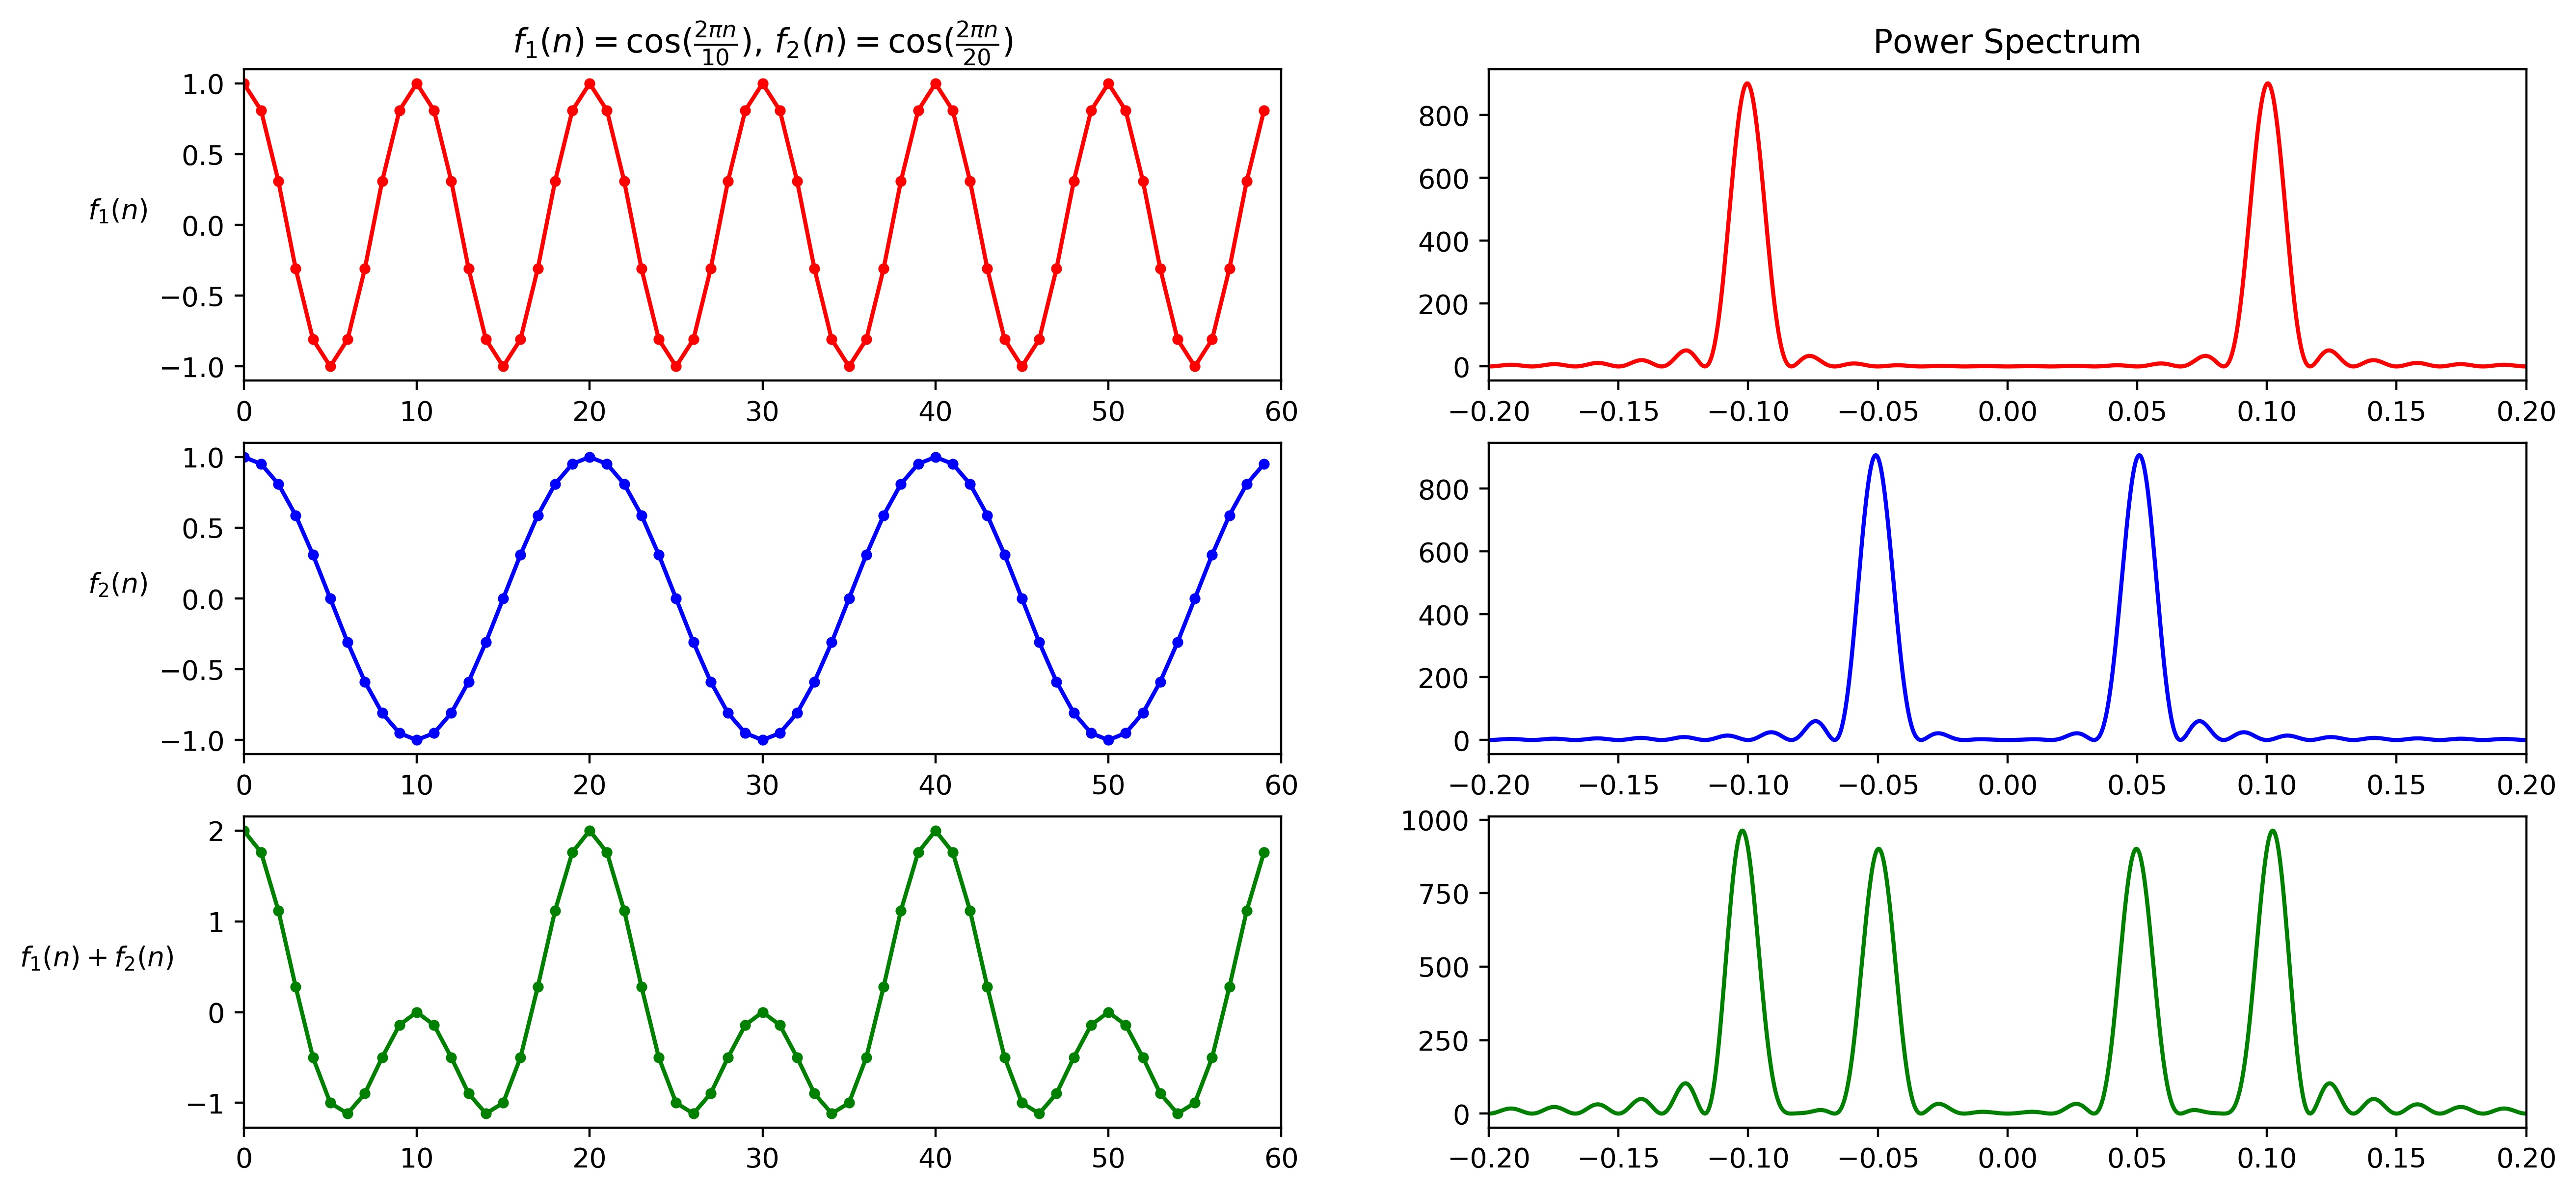
\includegraphics{Figuras/ft_exemplo.jpg}}
	\end{center}
	\vspace{1mm}	% acrescentar o espaçamento vertical apropriado entre a borda inferior da figura e a legenda ou a fonte quando não há legenda (o valor pode ser negativo para subir)
	\legenda{Esquerda: funções $f_{1}$ (no topo, de frequência 0.1), $f_{2}$ (no meio, de frequência 0.5) e uma combinação destas (abaixo). Direita: espectro de potência dos respectivos sinais à esquerda. O último plot evidencia a característica linear da FT, onde a soma dos sinais resultou num espectro de potência com duas assinaturas de frequência, correspondentes às assinaturas individuais dos sinais $f_{1}$ e $f_{2}$.}	% legenda - para deixar sem legenda usar comando \legenda{} (nunca deve-se comentar o comando \legenda)
	\label{fig:FT_exemplo}
	%\FONTE{\url{https://omniweb.gsfc.nasa.gov/form/dx1.html}.}	% fonte consultada (elemento obrigatório, mesmo que seja produção do próprio autor)
\end{figure}

Para a análise espectral dos dados de F10.7, foi utilizada a biblioteca \texttt{Numpy} do \texttt{Python}, com a rotina \texttt{fft} para computar a Transformada Discreta de Fourier. Baseada no algoritmo FFT (Fast Fourier  Transform), ela explora a simetria dos termos calculados e computa a DFT de forma eficiente \cite{cooley1965algorithm}. Conforme o manual, a função \texttt{numpy.fft.fft}, particularmente utilizada  nesta análise, fornece a transformada não normalizda. Se \texttt{A = fft(input)}, o primeiro termo do output \texttt{A[0]} é o de frequência zero, ou seja, a soma do sinal. \texttt{A[1:n/2]} contém os termos de frequência positiva e \texttt{A[n/2+1:]} contém os termos de frequência negativa. O espectro de potência é obtido fazendo-se \texttt{numpy.abs(A)**2}. Tais informações foram usadas para gerar a Figura \ref{fig:FT_exemplo} e também os resultados apresentados na próxima seção.
 %% 3o capítulo

%%%%%%%%%%%%%%%%%%%%%%%%%%%%%%%%%%%%%%%%%%%%%%%%%%%%%%%%%%%%%%%%%%%%%%%%%%%%%%%

\chapter{RESULTADOS E DISCUSSÃO}

A Figura \ref{fig:result} é o resultado da aplicação da FFT sobre os dados de F10.7. O espectro de potência produzido é exibido normalizado pelo tamanho da série, e somente metade dos coeficientes é mostrado (visto que o output é simétrico). A Figura \ref{fig:result_t} é o mesmo resultado em função do tempo.

\begin{figure}[ht!]
	\caption{Resultado da análise espectral.}
	\vspace{1mm}	% acrescentar o espaçamento vertical apropriado entre o título e a borda superior da figura
	\begin{center}
		\resizebox{\textwidth}{!}{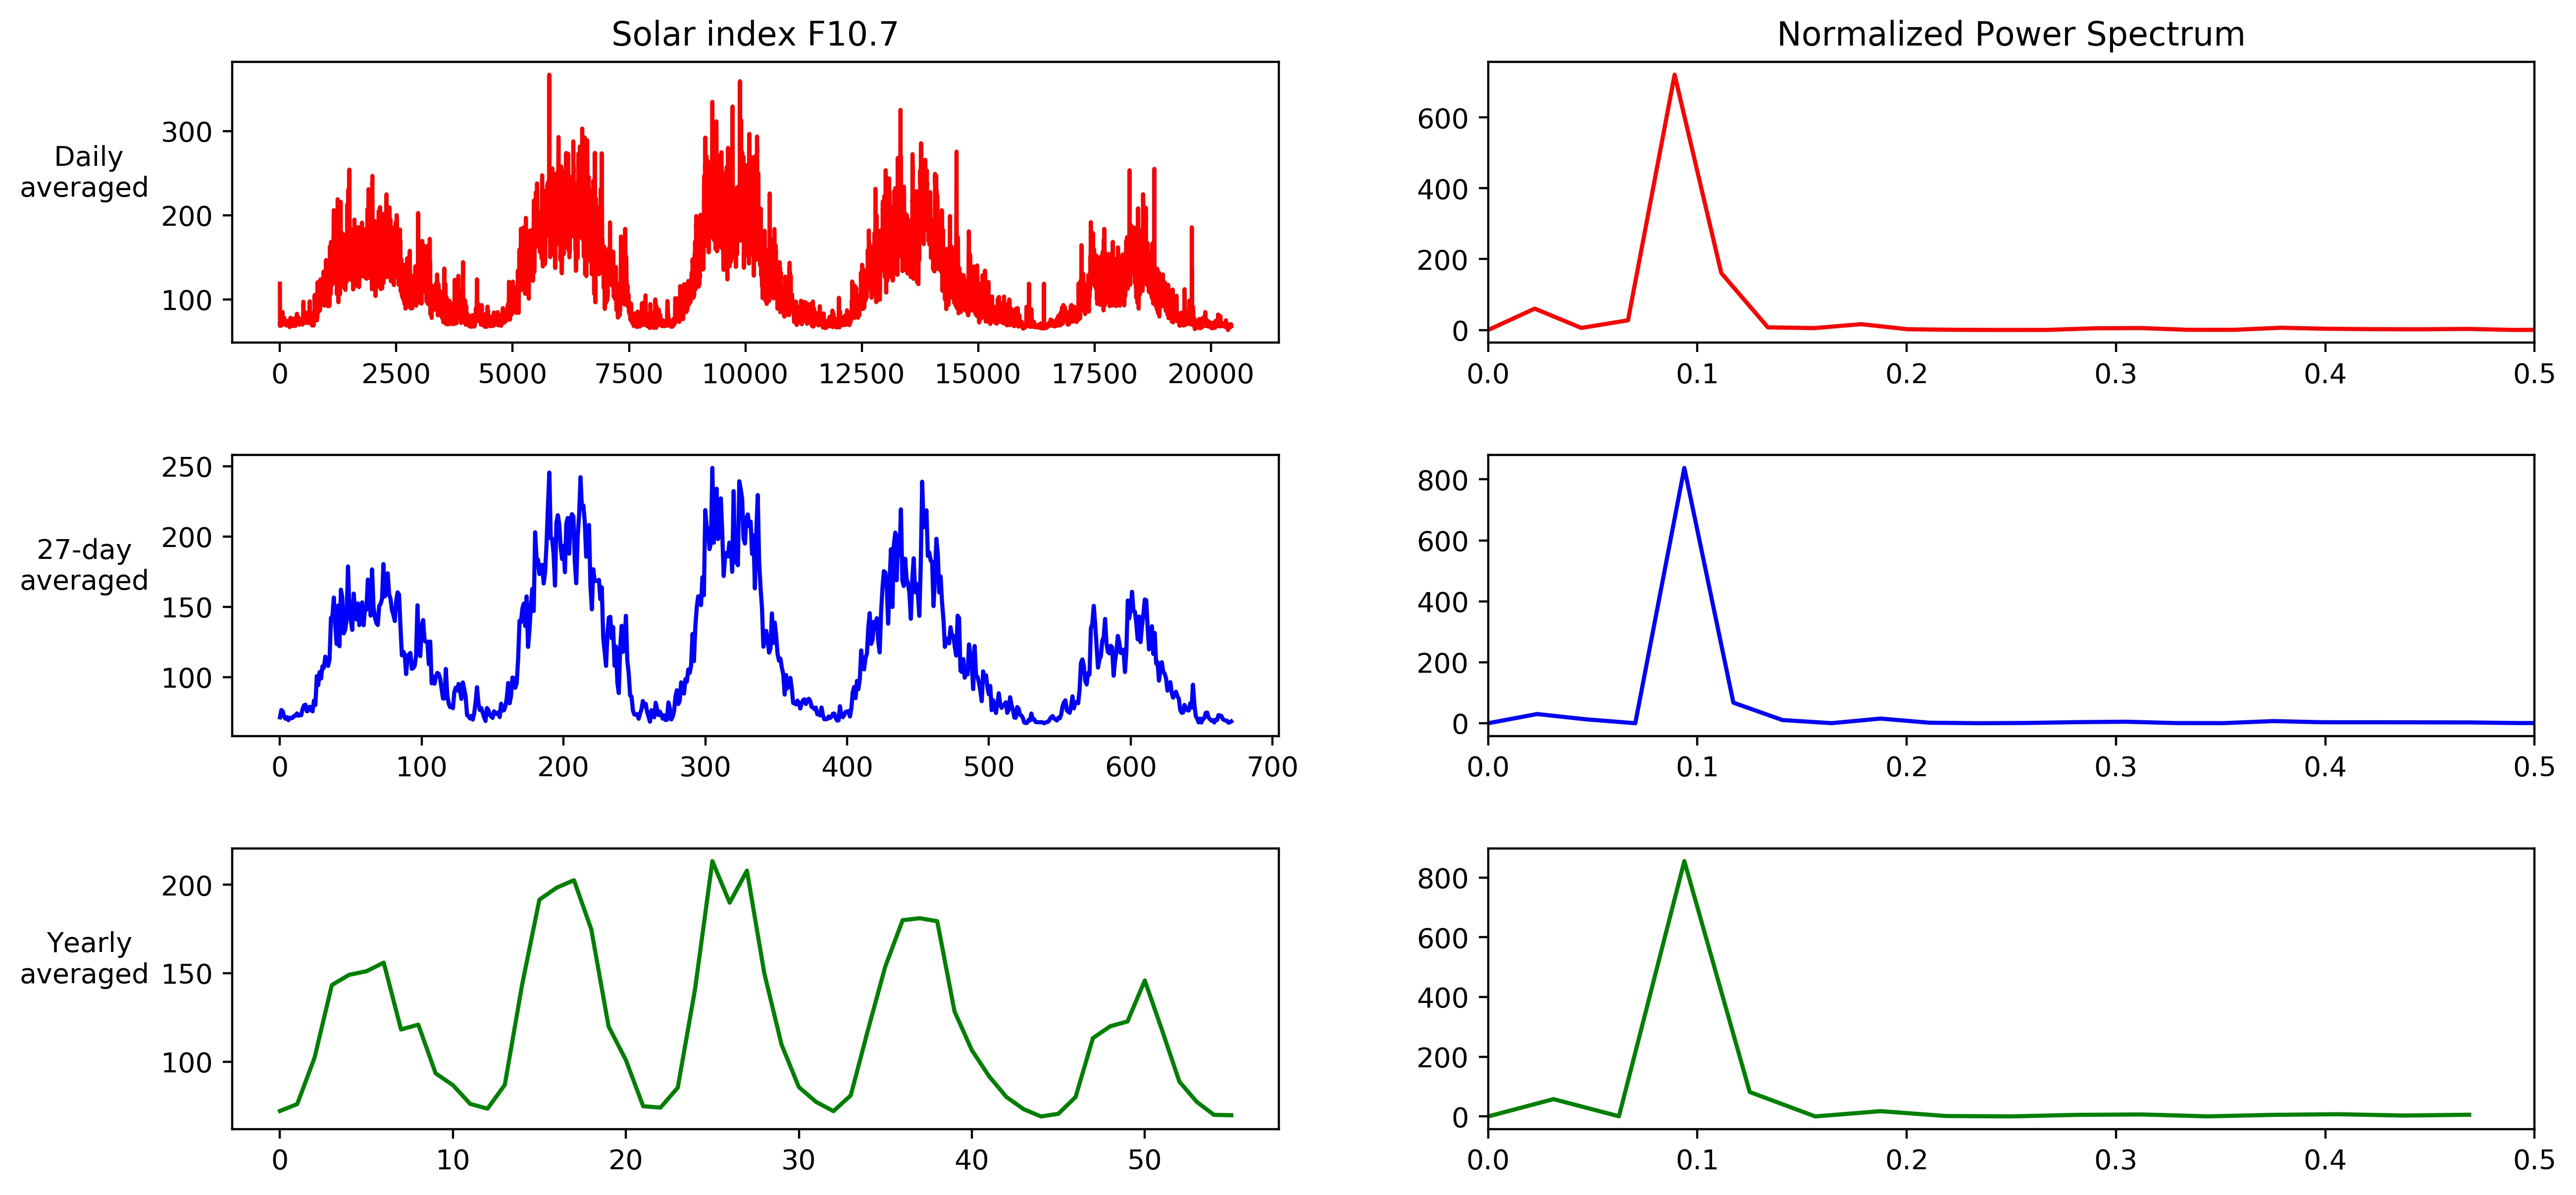
\includegraphics{Figuras/final_f.jpg}}
	\end{center}
	\vspace{1mm}	% acrescentar o espaçamento vertical apropriado entre a borda inferior da figura e a legenda ou a fonte quando não há legenda (o valor pode ser negativo para subir)
	\legenda{À esquerda, dados do fluxo solar com média diária (vermelho, cima), de 27 dias (azul, meio) e anual (verde, abaixo). À direita, resultado do espectro de potência normalizado dos respectivos sinais à esquerda. Somente metade dos coeficientes são exibidos, visto que o output é simétrico. O resultado indica que o pico da atividade solar ocorre em frequências baixas (em ciclos mais longos que um ano).}	% legenda - para deixar sem legenda usar comando \legenda{} (nunca deve-se comentar o comando \legenda)
	\label{fig:result}
	%\FONTE{\url{https://omniweb.gsfc.nasa.gov/form/dx1.html}.}	% fonte consultada (elemento obrigatório, mesmo que seja produção do próprio autor)
\end{figure}

\begin{figure}[ht!]
	\caption{Resultado em função do tempo.}
	\vspace{1mm}	% acrescentar o espaçamento vertical apropriado entre o título e a borda superior da figura
	\begin{center}
		\resizebox{\textwidth}{!}{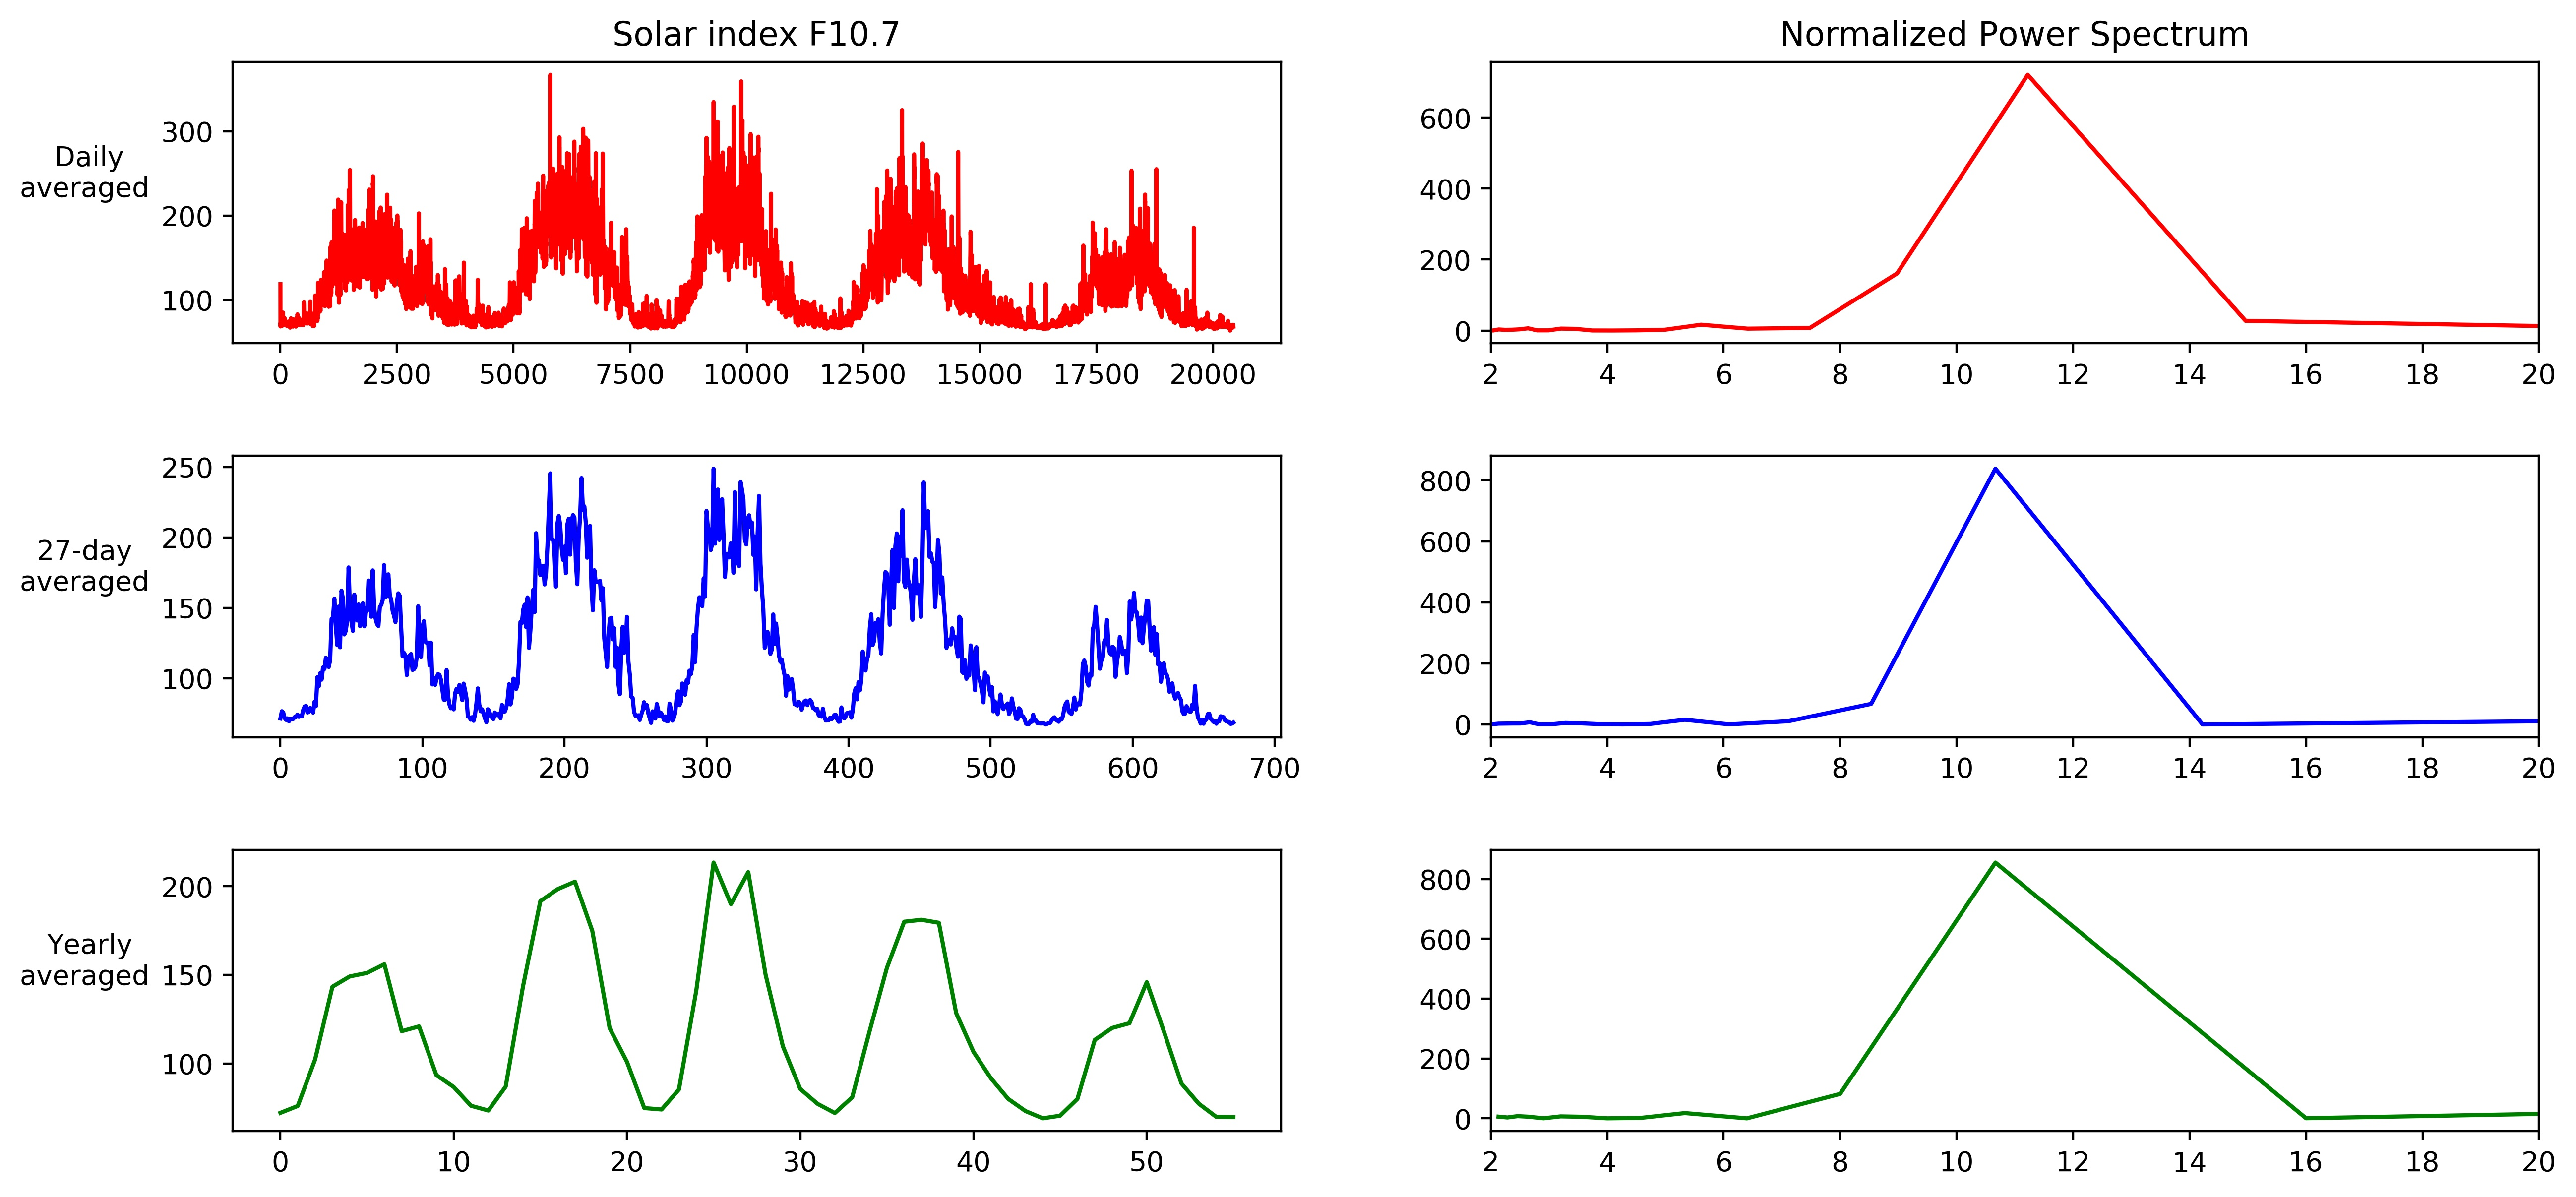
\includegraphics{Figuras/final_t2.jpg}}
	\end{center}
	\vspace{1mm}	% acrescentar o espaçamento vertical apropriado entre a borda inferior da figura e a legenda ou a fonte quando não há legenda (o valor pode ser negativo para subir)
	\legenda{Espectro de potência em função do período. O pico de atividade solar ocorre aproximadamente a cada onze anos.}	% legenda - para deixar sem legenda usar comando \legenda{} (nunca deve-se comentar o comando \legenda)
	\label{fig:result_t}
	%\FONTE{\url{https://omniweb.gsfc.nasa.gov/form/dx1.html}.}	% fonte consultada (elemento obrigatório, mesmo que seja produção do próprio autor)
\end{figure}

A principal diferença entre os três conjuntos de dados explorados está no tamanho da série. Por representarem o mesmo período temporal, pode-se interpretar que são registros do mesmo fenômeno em diferentes taxas de aquisição de dados (ou \textit{sampling}). Uma análise da Figura \ref{fig:result} indica que a média diária, o conjunto de dados de maior tamanho (2$^{14}$ entradas após tratamento) foi capaz de indicar a assinatura de frequências do sinal tão bem quanto os demais conjuntos (a média de 27 dias teve seu tamanho reduzido para 2$^{9}$ registros e a média anual para 2$^{5}$ após os procedimentos de tratamento discutidos na Seção 2). Isto deve-se ao fato de que todos os dados fazem parte de uma série histórica longa o suficiente (55 anos) para captar a assinatura do ciclo, e por isso a análise espectral é igualmente robusta para os três conjuntos analisados. E, conforme esperado, os resultados da Figura \ref{fig:result_t} indicam um ciclo de aproximadamente onze anos da atividade solar, um valor verificado na literatura e obtido também através da análise da variação do número de manchas solares. 
 %% 4o capítulo

%%%%%%%%%%%%%%%%%%%%%%%%%%%%%%%%%%%%%%%%%%%%%%%%%%%%%%%%%%%%%%%%%%%%%%%%%%%%%%%

\chapter{CONSIDERAÇÕES FINAIS}

As atividades realizadas no presente trabalho tiveram como objetivo solidificar os conceitos pertinentes à análise de sinais temporais. As ferramentas da Análise de Fourier foram aplicadas em dados de fluxo solar na faixa de 10.7 cm, que indicam a atividade solar cujo ciclo é conhecido e igual a onze anos. Dados de diferentes tamanhos referentes ao mesmo período temporal foram adquiridos e, em seguida: (1) explorados para familiarização e identificação de inconsistências; (2) tratados de maneira pertinente à análise espectral e (3) analisados com a rotina \texttt{numpy.fft} do \texttt{Python}. 

A rotina \texttt{numpy.fft} forneceu a Transformada Discreta de Fourier através do algoritmo FFT (Fast Fourier Transform). O resultado foi utilizado para gerar o espectro de potência. As Figuras 4.1 e 4.2 sugerem que a análise foi capaz de apontar o ciclo de período esperado (onze anos). Tais resultados indicam que as ferramentas utilizadas foram assimiladas de maneira satisfatória.
 %% 5o capítulo

%\include{./docs/capitulo6} %% 6o capítulo


%% insira quantos capítulos desejar com o seguinte comando:
%\include{_pasta_do_arquivo_/_meu_arquivo_} %%sem a extensão
%% note que deverá haver um arquivo _meu_arquivo_.tex (com extensão) no diretório _pasta_do_arquivo_

%\include{./docs/conclusao}

\newpage
%% Bibliografia %% não alterar %% obrigatório %testebib
\bibliography{./bib/referencia} %% aponte para seu arquivo de bibliografia no formato bibtex (p.ex: referencia.bib)


%\include{./docs/glossario} %% insira os termos do glossário no arquivo glossario.tex %% opcional

%\inicioApendice %% opcional, comente esta linha e a seguintes se não houver apendice(s)
%\include{./docs/apendice1} %% insira apendices tal qual capítulos acima


%\inicioAnexo
%\include{./docs/anexo}
%\include{./docs/anexo1}
%\include{./docs/anexo2}

%\inicioIndice
%\include{./docs/contracapa}
\end{document}